\documentclass[11pt]{article}
%\usepackage[14pt]{extsizes} % для того чтобы задать нестандартный 14-ый размер шрифта
%\usepackage[utf8]{inputenc}
\usepackage{mathtext}
\usepackage[english, russian]{babel}
\usepackage{amsmath}
\usepackage{amsfonts}
\usepackage{float}
\usepackage[margin=0.8in]{geometry}
\usepackage{multirow}
\usepackage{graphicx}
\usepackage[utf8x]{inputenc} % указать кодировку русского текста
\usepackage{fancyhdr}
\usepackage{indentfirst} % отступ в первой строке абзаца
\usepackage{wrapfig}
\usepackage{placeins}
\usepackage{wrapfig}
\usepackage{caption}
\usepackage{amssymb}
\usepackage{mathtools}
\usepackage[thinc]{esdiff}
\usepackage{cmap}
\usepackage[table,xcdraw]{xcolor}
\usepackage{icomma}

\pagestyle{fancy}
\begin{document}
\begin{titlepage}
\begin{center}
%\vspace*{1cm}
\large{\small ФЕДЕРАЛЬНОЕ ГОСУДАРСТВЕННОЕ АВТОНОМНОЕ ОБРАЗОВАТЕЛЬНОЕ\\ УЧРЕЖДЕНИЕ ВЫСШЕГО ОБРАЗОВАНИЯ\\ МОСКОВСКИЙ ФИЗИКО-ТЕХНИЧЕСКИЙ ИНСТИТУТ\\ (НАЦИОНАЛЬНЫЙ ИССЛЕДОВАТЕЛЬСКИЙ УНИВЕРСИТЕТ)\\ ФИЗТЕХ-ШКОЛА РАДИОТЕХНИКИ И КОМПЬЮТЕРНЫХ ТЕХНОЛОГИЙ}
\vfill
\line(1,0){430}\\[1mm]
\huge{Лабораторная работа 3.4.5}\\
\huge\textbf{Петля Гистерезиса (динамический метод)}\\
\line(1,0){430}\\[1mm]
\vfill
\begin{flushright}
\normalsize{Устюжанина Мария}\\
\normalsize{\textbf{Группа Б01-107}}\\
\end{flushright}
\end{center}
\end{titlepage}
\fancyhead[L] {Работа 3.4.5}

\par \textbf{Цель работы:} изучение петель гистерезиса различных ферромагнитных
материалов в переменных полях.

\par \textbf{В работе используются:} автотрансформатор, понижающий трансформатор, интегрирующая цепочка, амперметр, вольтметр, электронный осциллограф, делитель напряжения, тороидальные образцы с двумя обмотками.


\section{Экспериментальная установка}

Схема установки изображена на рис. $\ref{fig:scheme}$. Напряжение сети (220 В,
50 Гц) с помощью трансформаторного блока Т, состоящего из регулировочного автотрансформатора и разделительного понижающего трансформатора, подаётся на намагничивающую обмотку $N_0$ исследуемого образца.


\begin{figure}[H]
\center{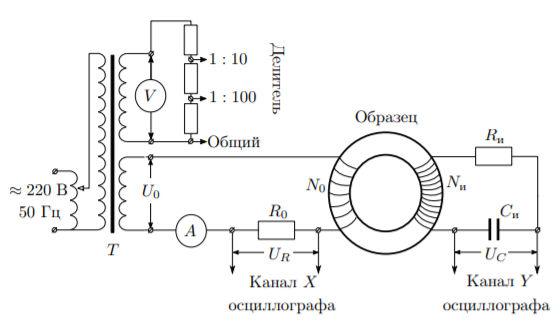
\includegraphics[scale=0.7]{scheme.png}}
\caption{Схема установки для исследования намагничивания образцов}
\label{pic:3}
\end{figure}

В цепь намагничивающей катушки, на которую подаётся некоторое
напряжение $U_0$, последовательно включено сопротивление $R_0$. Напряжение на $R_0$, равное $U_R$= $R_0I_0$, где $I_0$ — ток в намагничивающей обмотке $N_0$, подаётся на канал $ X $ осциллографа. Связь напряжённости $ H $ в
образце и тока $I_0$ рассчитывается по теореме о циркуляции. 
Действующее значение переменного тока в обмотке $N_0$ измеряется амперметром A.
Для измерения магнитной индукции $ B $ с измерительной обмотки $N_\text{и}$
на вход $ RC $-цепочки подаётся напряжение $U_\text{и}$ ($U_{\text{вх}}$), пропорциональное
производной $ dB/dt $. С интегрирующей ёмкости $C_\text{и}$ снимается напряжение $U_C$ ($U_{\text{вых}}$), пропорциональное величине $ B $, и подаётся на вход $ Y $
осциллографа. Значение индукции поля $ B $ рассчитывается по формуле ($\ref{eq:|B|new}$).
Замкнутая кривая, возникающая на экране, воспроизводит в некотором масштабе (различном для осей $ X $ и $ Y $) петлю гистерезиса. Чтобы придать этой кривой количественный смысл, необходимо установить
масштабы изображения, т. е. провести калибровку каналов $ X $ и $ Y $ осциллографа.



\section{Ход работы}

\subsection{Измерение петли гистерезиса}

\begin{enumerate}

\itemСоберем схему, подключаем в сеть. Параметры установки $R_\text{и} = 20~\text{кОм}, C_\text{и} = 20~\text{мкФ}, R_0 = 0.2~\text{Ом}$. Параметры образцов:
\begin{table}[h]
\centering
\begin{tabular}{|c|c||c||c|}
\hline
      &  Кремнистое железо  & Феррит   &  Пермаллой \\ \hline
$N_0$, витков    & 20            & 42        & 15                \\ \hline
$N_\text{и}$, витков    & 200           & 400       & 300               \\ \hline
$S$, см$^2$     & 2        & 3  & 0,66            \\ \hline
$2\pi R$, cм & 11          & 25      & 14,1              \\ \hline
\end{tabular}
\end{table}



\item Подбираем ток питания и коэффициенты усиления ЭО так, чтобы предельная петля гистерезиса занимала большую часть экрана.

\item Снимаем начальную кривую намагничивания: плавно уменьшая ток намагничивания до нуля, будем отмечать вершины наблюдаемых частных петель. Кривая, соединяющая эти вершины, проходит вблизи начальной кривой намагничивания. 

\begin{table}[h]
\centering
\begin{tabular}{|c|c||c||c|}
\hline
      &  Кремнистое железо  & Феррит   &  Пермаллой \\ \hline
$K_X$, B/дел    & 0,19            & 0,048        & 0,048                \\ \hline
$K_Y$, B/дел    & 0,038           & 0,015       & 0,038               \\ \hline
$I$, A     & 2.24             & 0.73  & 0,66            \\ \hline
\end{tabular}
\end{table}




\item По экрану ЭО измеряю полную ширину и высоту предельных петель - $2X_s$ и $2Y_s$, соответствующие удвоенной амплитуде колебания напряженности $H_s$ и индукции $B_s$ поля в образце в состоянии насыщения.

\begin{figure}[H]
\center{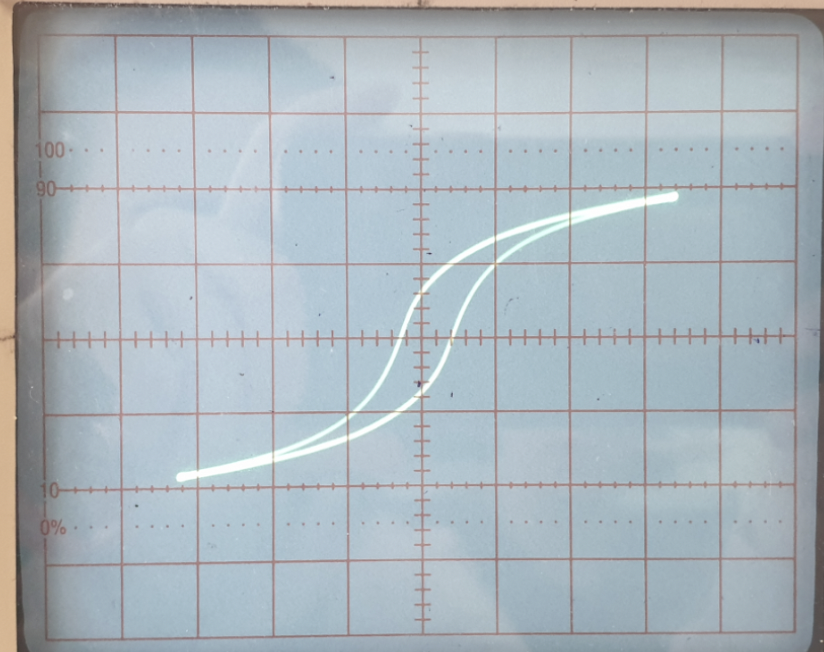
\includegraphics[scale=0.7]{photo1.png}}
\caption{Петля гистрезиса для кремниего железа}
\label{pic:3}
\end{figure}

\begin{figure}[H]
\center{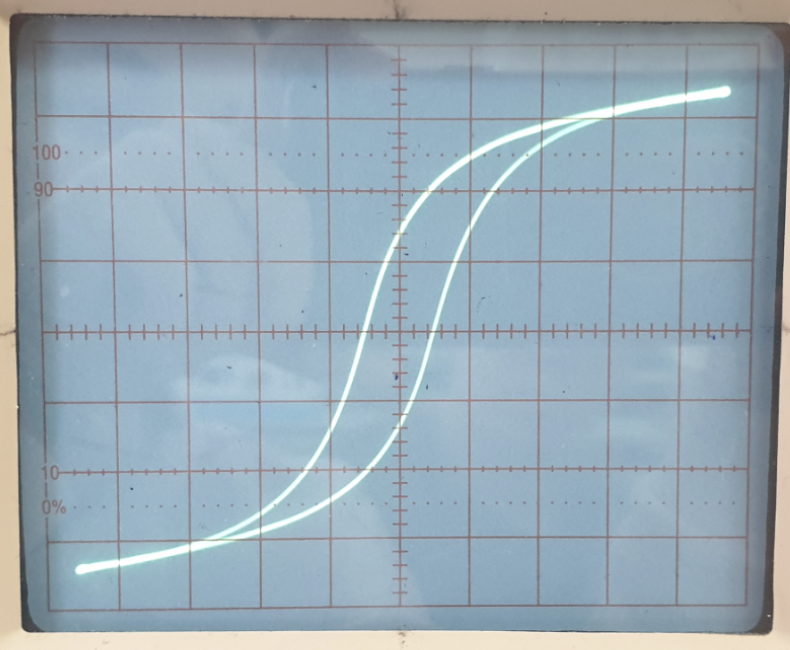
\includegraphics[scale=0.7]{photo2.png}}
\caption{Петля гистрезиса для феррита}
\label{pic:3}
\end{figure}

\begin{figure}[H]
\center{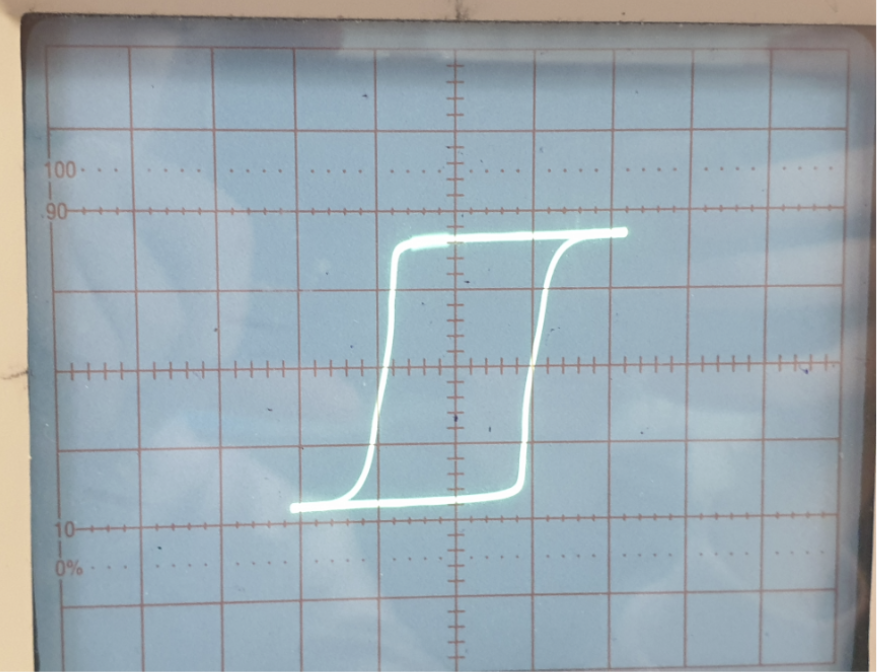
\includegraphics[scale=0.7]{photo3.png}}
\caption{Петля гистрезиса для пермвллоя}
\label{pic:3}
\end{figure}


\item Также измерим $2X_c$ - ширина петли на пересечении с осью абсцисс и $2Y_c$ - высота петли на пересечении с осью ординат.



Значения, полученные в пунктах 4 - 5 представлены в таблице:

\begin{table}[h] 
\centering
\begin{tabular}{|l|c|c|c|}
\hline
          & \multicolumn{1}{l|}{Кремнистое железо} & \multicolumn{1}{l|}{Феррит} & \multicolumn{1}{l|}{Пермаллой} \\ \hline
$2X_s, дел$ & 7                                      & 9                          & 4,2                             \\ \hline
$2Y_s, дел$ & 3,9                                     & 6,8                          & 3,6                             \\ \hline
$2X_c, дел$ & 0,7                                      & 1                          & 1,8                             \\ \hline
$2Y_c, дел$ & 1,4                                     & 2,8                          & 3,4                             \\ \hline
\end{tabular}
\end{table}



\subsection{Определение параметров RC-ячейки}

\item Измерим постоянную времени RC-ячейки. Для этого разберем цепь тороида и подадим на вход ячейки синусоидальное напряжение с обмотки $U_0$ понижающего трансформатора. 
Подключим Y-вход ЭО ко входу интегрирующей ячейки и отключим Х-вход ЭО. Определим входное напряжение на RC-цепочке: $U_{\text{вх}} = 4,26 \text{В}$.
Не меняя тока, переключим Y-вход ЭО к выходу ячейки  и аналогичным образом определим напряжение $U_{\text{вых}}= 0,033 \text{В}$. Тогда (с учётом $\nu = 50~\text{Гц}$)
\begin{center}
\fbox{$\tau = \dfrac{U_\text{вх}}{\omega U_\text{вых}} = 0.41 ~\text{с}$}
\end{center}
Рассчитывая через параметры цепи, $\tau = R_\text{и} C_\text{и} = 0.4~\text{c}$, что почти равно полученному.

\subsection{Обработка результатов}
\item  Рассчитаем коэрцитивную силу и индукцию насыщения для каждого образца и сравним с табличными. При расчетах будем использовать формулы связи напряженности и тока в тороидальном образце : $H = \frac{IN_0}{2\pi R}$ и результаты калибровки канала Х.

Цена деления:
$h = \frac{K_xN_0}{2\pi R R_0}$
$b = \frac{K_yR_uC_u}{S N_u}$

Умножая $X_c$ на h получаем $H_c$, аналогично $B_s$ - это $Y_s$ умноженное на b.
Полученные h и b для всех образцов:

\begin{table}[h]
\centering
\begin{tabular}{|l|c|c|c|}
\hline
           & \multicolumn{1}{l|}{Кремнистое железо} & \multicolumn{1}{l|}{Феррит} & \multicolumn{1}{l|}{Пермаллой} \\ \hline
h, A/м дел & 1,72                                  & 40,3                        & 25,5                           \\ \hline
b, Тл/дел  & 0,38                                   & 0,05                        & 0,77                          \\ \hline
\end{tabular}
\end{table}


Полученные значения для $H_c$ и $B_s$:

\begin{table}[h]
\centering
\begin{tabular}{|l|c|c|c|}
\hline
           & \multicolumn{1}{l|}{Кремнистое железо} & \multicolumn{1}{l|}{Феррит} & \multicolumn{1}{l|}{Пермаллой} \\ \hline
$H_c$, A/м & 
60                                  & 20,15                        & 22,9                           \\ \hline
$Табл H_c$, A/м & 
40                                  & 4-100                        & 5,6                           \\ \hline
$B_s$, Тл  & 
0,133                                   & 0,07                        & 
1,31                          \\ \hline
$Табл B_s$, Тл  & 1,95                                   & 0,1-0,4                        & 1,05 - 1,6                          \\ \hline
\end{tabular}
\end{table}



\begin{center}
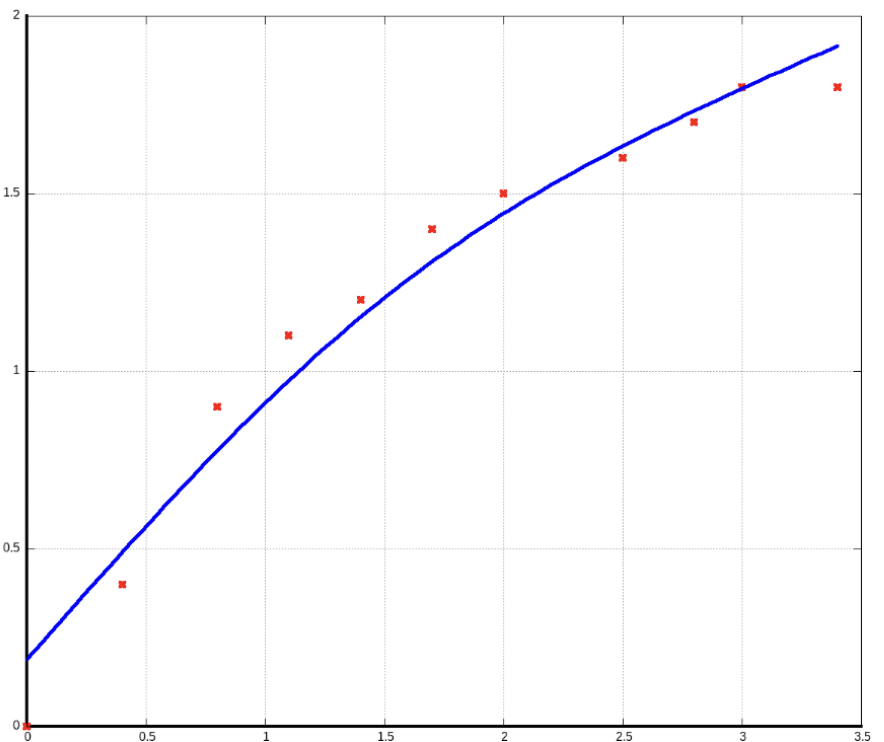
\includegraphics[scale=1]{graf1.png}
\end{center}

\begin{center}
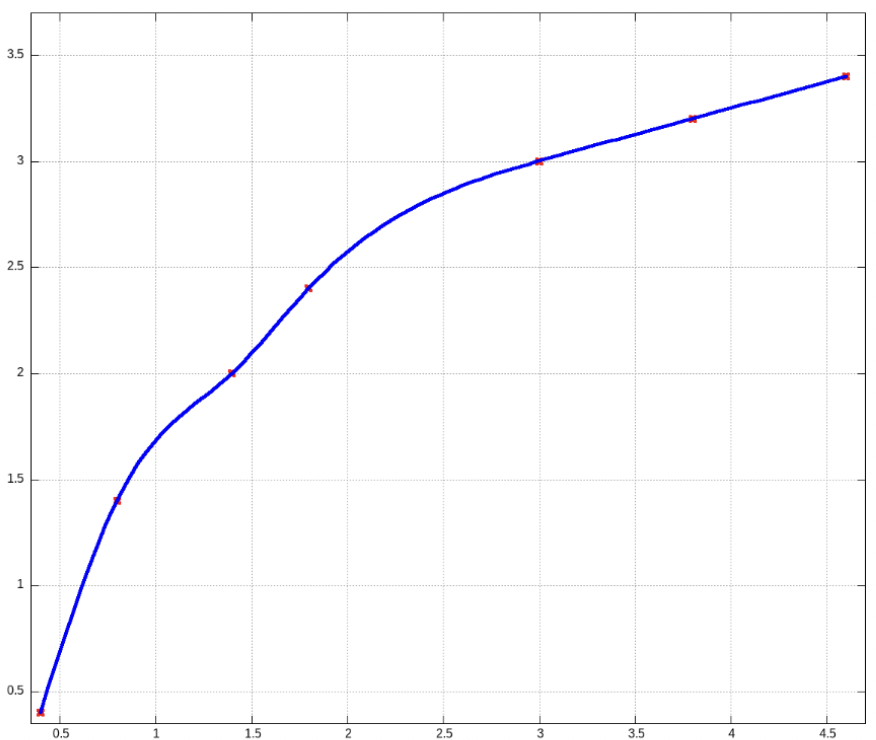
\includegraphics[scale=1]{graf2.png}
\end{center}

\begin{center}
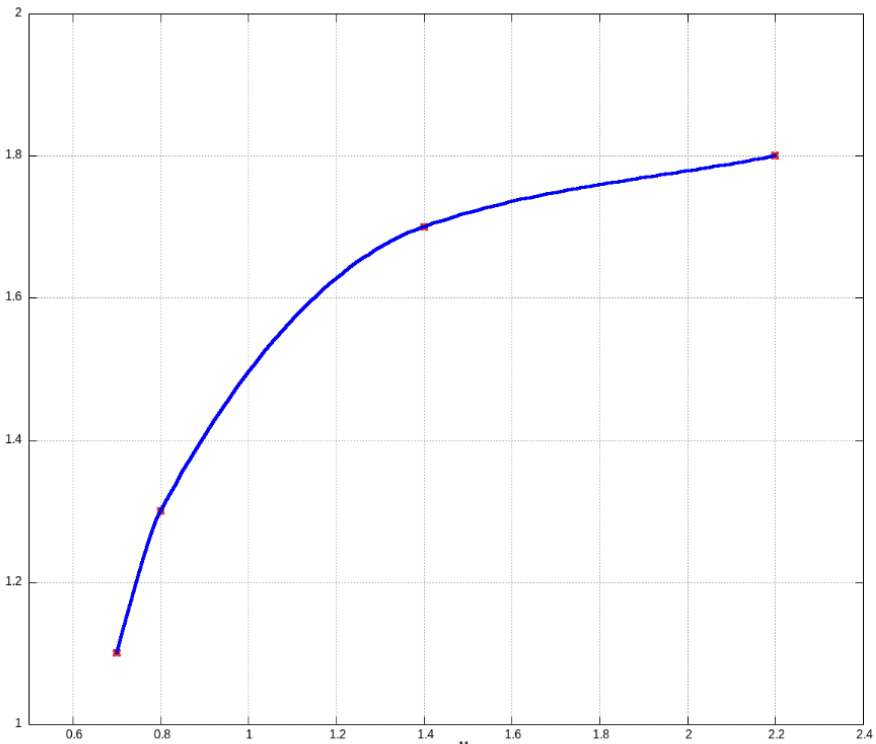
\includegraphics[scale=1]{graf3.png}
\end{center}

Полученные значения $\mu_{диф}$:
\begin{table}[h]
\centering
\begin{tabular}{|l|c|c|c|}
\hline
                      & \multicolumn{1}{l|}{Кремнистое железо} & \multicolumn{1}{l|}{Феррит} & \multicolumn{1}{l|}{Пермаллой} \\ \hline
$\mu_{нач} - \mu_{max}$ &     $(3980 - 5175)\pm 800$                                   & $       9010\pm 500$                     &$              1700\pm 760                 $ \\ \hline
табличные значения    & 500-7000                               & 500-20000                   & 1200-3500                      \\ \hline
\end{tabular}
\end{table}


\end{enumerate}




\section{Выводы}

Т. к. в работе присутствует осциллограф, практически все погрешности определяются погрешностью, связанной со снятием показаний по экрану. Т. к. физически невозможно считать показания лучше, чем с точностью 1/10 дел., погрешность $ h $ и $ b $ 10\%. 

В работе я получила начальные кривые намагничивания, нашла значения $B_s$ и $H_c$, сравнила с табличными, нашла $\mu_{диф}$ и постоянную времени RC-ячейки $\tau$. Полученные значения получились близки к табличным, кроме пермаллоя, там есть небольшое отклонение.



\end{document}